\documentclass[10pt,a4paper]{article}
\usepackage[utf8]{inputenc} % para poder usar tildes en archivos UTF-8
\usepackage[spanish]{babel} % para que comandos como \today den el resultado en castellano
\usepackage{a4wide} % márgenes un poco más anchos que lo usual
\usepackage[conEntregas]{caratula2}
\usepackage{float}
\usepackage[pdftex]{graphicx}
\usepackage{caption}
\usepackage{subcaption}
\usepackage{amsmath,amssymb}
\usepackage{algorithm}
\usepackage{algpseudocode}
\usepackage{pifont}

%Esto de abajo es para encabezado y pie de pagina
\usepackage{lastpage}
\usepackage{fancyhdr}
\usepackage{ulem}
% Simbolos matemáticos
%\usepackage{amsmath}
%\usepackage{amsfonts}
%\usepackage{amssymb}
%\usepackage{algorithm}
%\usepackage{algpseudocode}
% Descoración y gráficos
%\usepackage{fancyhdr}
%\usepackage{multirow}
%\usepackage{alltt}
\usepackage{listings}
\usepackage{color}

\definecolor{mygreen}{rgb}{0,0.6,0}
\definecolor{mygray}{rgb}{0.5,0.5,0.5}
\definecolor{mymauve}{rgb}{0.58,0,0.82}

\lstset{ %
  backgroundcolor=\color{white},   % choose the background color; you must add \usepackage{color} or \usepackage{xcolor}
  basicstyle=\footnotesize,        % the size of the fonts that are used for the code
  breakatwhitespace=false,         % sets if automatic breaks should only happen at whitespace
  breaklines=true,                 % sets automatic line breaking
  frame=single,                    % adds a frame around the code
  keepspaces=true,                 % keeps spaces in text, useful for keeping indentation of code (possibly needs columns=flexible)
  keywordstyle=\color{blue},       % keyword style
  language=SQL,                 % the language of the code
  numbers=left,                    % where to put the line-numbers; possible values are (none, left, right)
  numbersep=5pt,                   % how far the line-numbers are from the code
  numberstyle=\tiny\color{mygray}, % the style that is used for the line-numbers
  rulecolor=\color{black},         % if not set, the frame-color may be changed on line-breaks within not-black text (e.g. comments (green here))
  showspaces=false,                % show spaces everywhere adding particular underscores; it overrides 'showstringspaces'
  showstringspaces=false,          % underline spaces within strings only
  showtabs=false,                  % show tabs within strings adding particular underscores
  stepnumber=1,                    % the step between two line-numbers. If it's 1, each line will be numbered
  stringstyle=\color{mymauve},     % string literal style
  tabsize=4,                       % sets default tabsize to 2 spaces
  title=\lstname                   % show the filename of files included with \lstinputlisting; also try caption instead of title
}

\pagestyle{fancy}

\cfoot{\thepage /\pageref{LastPage} }



\newcommand\BlockIf[1]{\KwSty{If} \\ #1 \\ \KwSty{End If}}
\newcommand\BlockElseIf[1]{\KwSty{Else If} \\ #1 \\ \KwSty{End Else If}}
\newcommand\BlockElse[1]{\KwSty{Else} \\ #1 \\ \KwSty{End Else}}

\begin{document}

\titulo{Trabajo Práctico}
\subtitulo{Sudoku}

\fecha{\today}

\materia{Metaheurísticas}
\submateria{2do Cuatrimestre de 2015}
%\grupo{Grupo 5}

\integrante{Kujawski, Kevin}{459/10}{kevinkuja@gmail.com}
\integrante{Ortiz de Zarate, Juan Manuel}{45/10}{jmanuoz@gmail.com}

% Pongan cuantos integrantes quieran

\maketitle

\newpage
\tableofcontents
%compilar varias veces si no se actualiza el indice o el pie de pagina

\newpage
\section{Introducción}
Sudoku es un juego de lógica cuyo objetivo es rellenar una cuadricula de tamaño 9x9, divididas a su vez en 9 cajas de 3x3, estas últimas llamadas cajas. Inicialmente contiene cierta cantidad de celdas con valores fijos pre-definidos y válidos, es decir, sus valores están entre [1,9], no hay repetidos por filas, columnas o cajas. \\Las reglas del juego son:
\begin{enumerate}
  \item Cada fila debe contener todos los números en el intervalo [1,9]
  \item Cada columna debe contener todos los números en el intervalo [1,9]
  \item Cada caja debe contener todos los números en el intervalo [1,9]
\end{enumerate}

El objetivo del juego es rellenar las celdas en blanco de la cuadricula inicial respetando las reglas del juego. A pesar de las simpleza del objetivo y las reglas del juego, hay 6670903752021072936960 formas posibles de ser rellenada una cuadricula. Buscar una solución intentando todas las formas posibles es claramente imposible, y eso incentiva la utilización de una metaheurística para solucionar el juego.\\
En el presente trabajo, presentaremos una posible formulación matemática del Sudoku como un problema de optimización e dos propuestas de implementación utilizando dos metaheurísticas: Simulated annealing y Colonia de hormigas

\section{Descripción y formulación matemática}


Nuestra formulación matemática es una adaptación de (2). En esa formulación, las variables $X_{ijk} $ son variables de decisión, definidas de la siguiente manera:
\[
X_{ijk}= \left\{ \begin{array}{lcc}
             1 &   $si el elemento (i,j) de la cuadricula contiene  el valor k$\\
             \\ 0 &  $en caso contrario$
             \end{array}
   \right.
   \]

   
  La formulación como programación lineal entera es la siguiente:	
\begin{equation*}
\begin{array}{ll@{}ll}
\text{min}  & \displaystyle $FuncionCosto(X)$ &\\
\text{sujeto a} & \displaystyle\sum\limits_{i=1}^{9} X_{ijk}=1, j=1:9,k=1:9 & (1)\\
		& \displaystyle\sum\limits_{j=1}^{9} X_{ijk}=1,i=1:9,k=1:9 & (2)\\
		& \displaystyle\sum\limits_{j=3q-2}^{3q} \sum\limits_{i=3p-2}^{3p} X_{ijk}=1, k=1:9,p=1:3,q=1:3 & (3) \\
                 & \displaystyle\sum\limits_{k=1}^{9} X_{ijk}=1, i=1:9,j=1:9 & (4)\\
                 & X_{ijk}=1 \forall (i,j,k) \in INICIALES &(5) \\
                 &  X_{ijk} \in {0,1}
\end{array}
\end{equation*}

 
 Hay que notar que como se trata de un problema de satisfacibilidad, la formulación no necesita de una función objetivo, por eso la definimos como 0. Las restricciones (1),(2) y (3) garantizan que cada numero en el intervalo posible de la instancia solo aparezca una vez en cada columna, fila, y caja, respectivamente. La restricción (4) garantiza que todas las posiciones de la martiz esten rellenas. La restricción (5) fuerza que las variables fijas de la instancia permanezcas sin alterar.


\newpage
\section{Descripci\'on de la Soluci\'on}

\subsection{Simulated annealing}
\subsubsection{Definición}
Simulated annealing (Recocido Simulado en español), respecto a las ciencias de la computación, es una metaheuristica para problemas de optimización global, aplicandose a la heurística de Búsqueda Local Aleatoria. La técnica fue presentada por Kirkpatrick, Gelatt y Vecci (1982) y ha sido
muy empleado para resolver problemas combinatorios.
La idea surge del proceso físico conocido como
recocido en el cual, se eleva la temperatura de un
sólido hasta el punto que se vuelve líquido, a continuación
la temperatura se disminuye de forma paulatina
para obtener una estructura cristalina sin defectos
y que puede considerarse como un estado de
mínima energía. Cada descenso de temperatura debe
ser lo suficientemente pequeño para que el sistema
no adquiera una estructura cristalina con defectos,
además el sistema debe permanecer un tiempo
suficiente a una misma temperatura para permitir
alcanzar un estado estacionario, en otras palabras,
que las partículas vuelvan a reacomodarse.


Se parte de una solución inicial posible $S_{i}$, luego se selecciona
una solución posible $S_{j}$ dentro de una vecindad, enseguida
se evalúa la calidad de la solución posible
empleando una función de costo f(x) asociada a cada posible solución S del problema.\\

Si la nueva solución posible $S_{j}$ es mejor que la actual
(de acuerdo al costo), se acepta, de lo contrario
se selecciona de acuerdo a una probabilidad, para
Simulated annealing dicha probabilidad de selección
está dada por la ecuación (1) que se conoce como
el criterio de Metropolis; a $temp$ se le conoce como
el parámetro de control; este valor se inicia con un valor
suficientemente grande para que cualquier solución
tenga una probabilidad alta de ser seleccionada,
a medida que $temp$ disminuye, la probabilidad de
aceptar soluciones factibles de mala calidad disminuye. El enfriamiento
se realiza empleando el sistema geométrico
dado por la ecuación (2), donde $\alpha$ es un parámetro
fijo.

\begin{equation*}
\begin{array}{ll@{}ll}
criterio(S_{i}, S_{j})= exp( (costo(S_{i}) - costo(S_{j})) / temp) & (1) 
\end{array}
\end{equation*}

\begin{equation*}
\begin{array}{ll@{}ll}
temp_{k+1} =  temp_{k} *  \alpha & (2)
\end{array}
\end{equation*}


\subsubsection{Implementación para resolver Sudoku}
Antes de ir directo al algoritmo hay que tener en cuenta las diferentes elecciones que hicimos para encontrar una solución inicial, mejorarla y  decidir cuando una solución es mejor que otra.
\paragraph{Solución inicial} 
Como el algoritmo así lo requiere, debemos partir de una solución inicial para intentar mejorarla y en el mejor de los casos poder resolverla. Una primera opción que se puede pensar es, a partir de las celdas iniciales, rellenar todas las celdas vacías con valores aleatorios directamente. Sin descartar totalmente esta idea fuimos un poco más allá. Básicamente intentamos resolver el Sudoku lo más que podamos, estando siempre seguro de que los valores que pongamos en las celdas son los correctos. Para esto analizamos los posibles valores que pueden ir en cada celda, eliminando de esas posibilidades valores que estén en la misma fila, columna o caja. Luego de esto, en caso de detectar que una celda tiene un solo valor posible, se rellenará la celda con ese valor y se lo considerará correcto ya que fue deducido de la configuración inicial. En caso de que no haya valores posibles para esa celda, indicará que esa configuración inicial no tiene solución posible. Por cada celda que se rellene se deberá recalcular todo el proceso de nuevo, hasta que en algún ciclo no haya modificaciones. \\Una vez que se terminó de deducir lo máximo posible será el momento de rellenar las celdas que quedaron vacias. Para este punto intentaremos ser lo menos aleatorio posible, y para tal caso seleccionaremos entre los posibles valores que pueden tener la celda, que ya habíamos calculado en el punto anterior. Y en caso de que para una celda ya no haya posibles valores, es el momento en que se le asignará uno aleatorio, siempre respetando la formulación (3) que se menciona en la sección anterior, es decir, se respetará en todo momento que no haya celdas inválidas en las cajas.
\paragraph{Función de costo}
El costo (o penalización) va a depender de la cantidad de celdas "ilegales" que tenga la cuadricula. Es decir, cuando haya una celda que se repita en la fila, columna o caja se sumará una penalidad. El caso ideal, que indica que el tablero está solucionado, es cuando el costo devuelve 0.
\paragraph{Soluciones vecinas}
\paragraph{Algoritmo}

\newpage
\section{Decisiones tomadas y su justificaci\'on}



\newpage
\section{Experimentos}

En primera instancia realizamos experimentos con ambas metaheurísticas a sudokus de distintos niveles de dificultad [3] y randoms (estos son sudokus solucionados a los que les blanqueamos de manera random 30 casillas). El objetivo es comparar los algoritmos entre sí para ver cuan efectivos son.


\begin{table}[ht]
\centering
\begin{tabular}{|l|l|l|}
\hline
          & \textbf{Simulated Annealing} & \textbf{Colonia de Hormigas} \\ \hline
{Escenarios probados} &       115                       &        115                      \\ \hline
{Total Solucionados} &                      70 (60\%)      &              60 (52\%)               \\ \hline
{Dificultad baja} &                     71 \%         &              69\%                \\ \hline
{Dificultad moderada} &                  40 \%            &             25 \%                 \\ \hline
{Dificultad alta} &                         16\%     &            5 \%                  \\ \hline
{Random} &                         63\%     &            60 \%                  \\ \hline
\end{tabular}
\end{table}



\subsection{Simulate annealing}
Para los experimentos elegimos un factor de enfriamiento en 0.5 y una temperatura inicial de 1. La justificación es en base a los experimientos realizados y que mostraremos en esta sección. \\ \\

El siguiente grafico es el resultado del tiempo que toma solucionar un Sudoku en donde partiendo de una solución existente blanqueamos celdas random y observamos como lo soluciona el algoritmo:\\
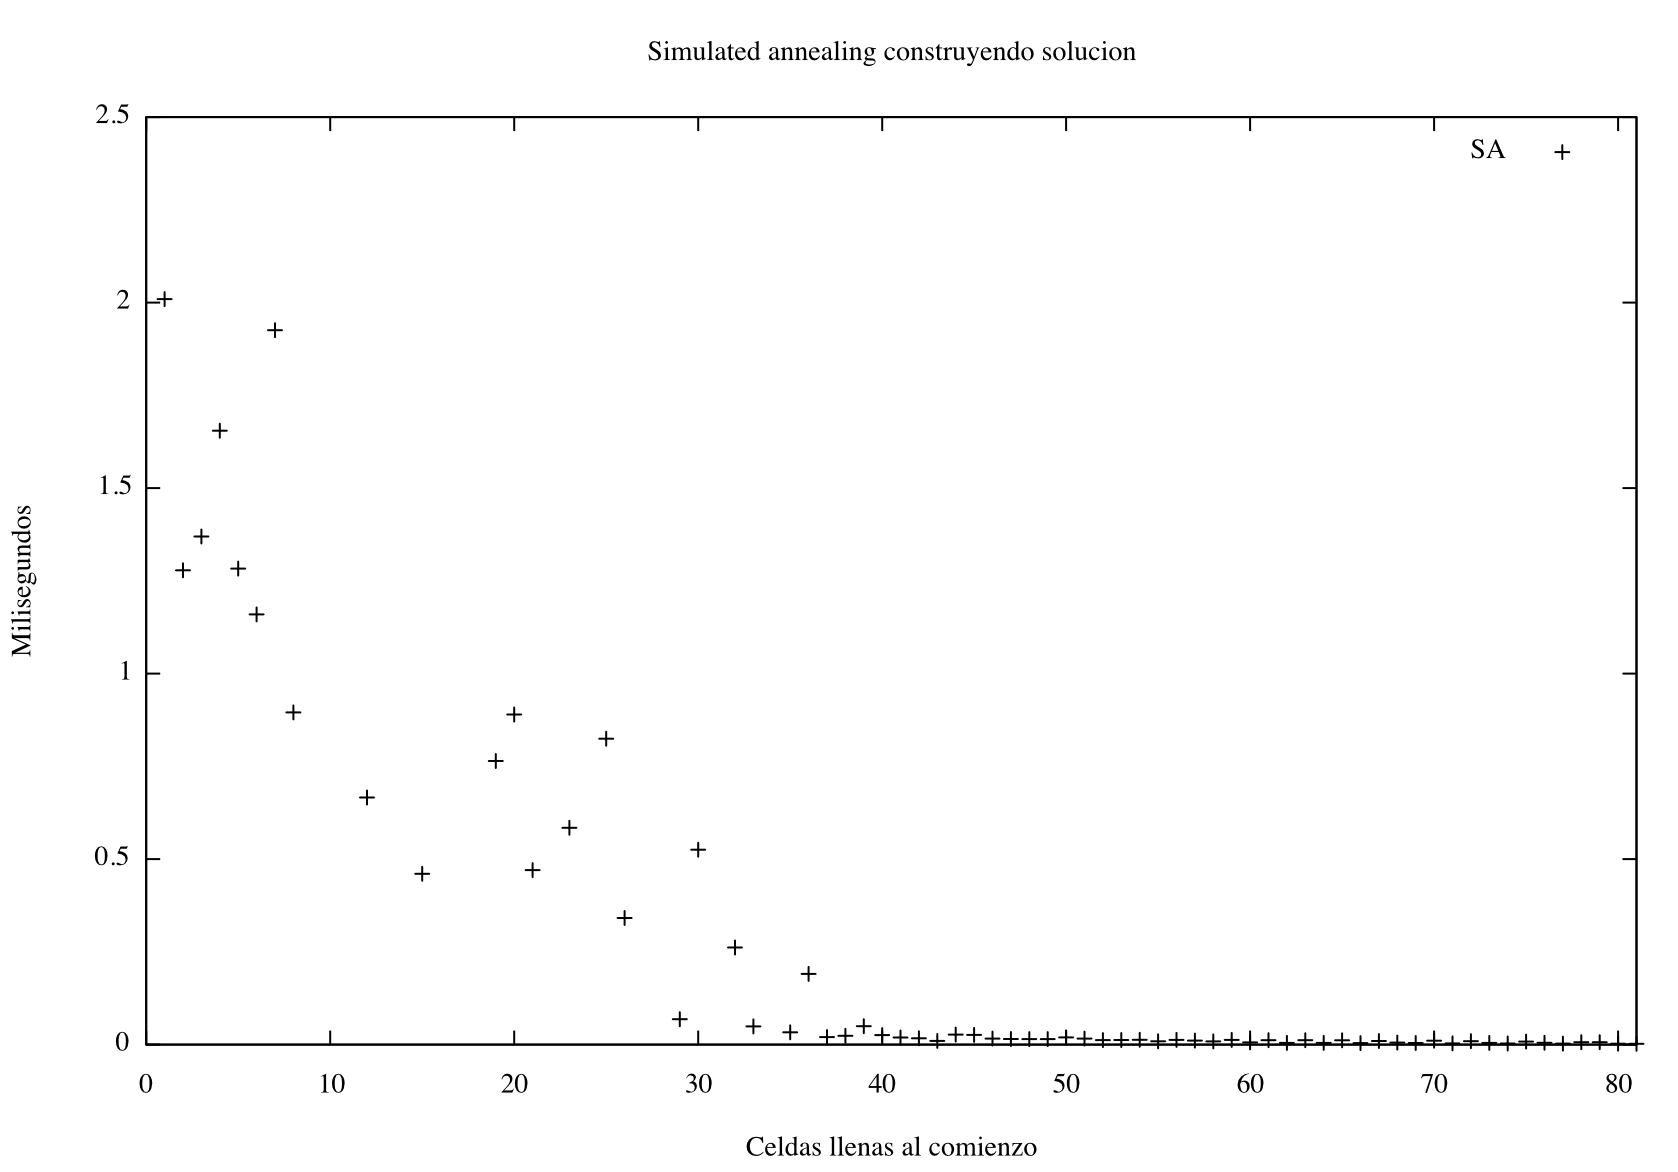
\includegraphics[scale=0.5]{imgs/randomSA.png}	\\
Clarmente se puede observar que a medida que el tablero esta mas lleno el tiempo es menor, eso es debido a la suma de varios factores, como que inicialmente infiere más celdas, son menos las vacias (que se convierte en menos iteraciones) y menos búsqueda de soluciones vecinas.\\\\

A continuación corrimos el algoritmo con 25 soluciones de diferentes niveles de dificultad, variando el factor de enfriamiento (o alfa):\\
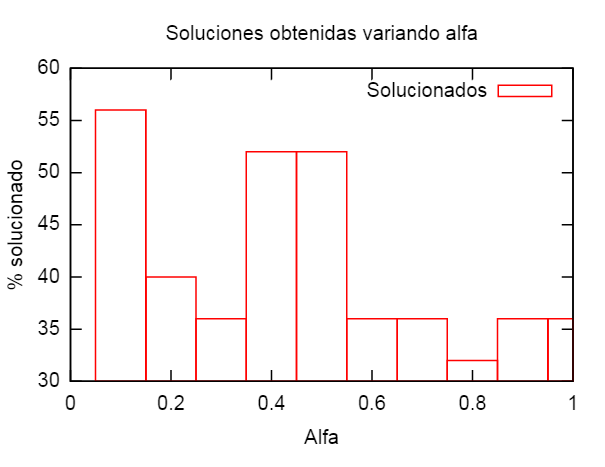
\includegraphics[scale=0.7]{imgs/porc_soluc.png}	\\
Si bien con valores intermedios (aprox 0.5) es donde se concentran las mejores soluciones, y que la mayor cantidad se logra con un 0.1, creemos en base a anteriores pruebas que el el factor de enfriamiento debería ser siempre mayor de 0.5 para que sea algo "lento" y no siempre elija ir por soluciones vecinas pero que tampoco las restrinja totalmente. 


\newpage
\section{Conclusiones}

En este trabajo, hemos presentado, a nuestro entender, dos aplicaciones de metaheurísticas para resolver el popular rompecabezas de 9x9 conocido como \textbf{Sudoku}. Hemos aplicado los algoritmos a distintos problemas tomados de sitios (de distintos grados de "dificultad"), y hemos visto en todas nuestras pruebas de que los algoritmos no llegan a conseguir cierta optimalidad (como suele ser el caso de las técnicas de optimización), logrando mejores resultados con el Simulated annealing respecto a la Colonia de Hormigas, pero consistentemente encuentran la solución en un tiempo razonable, ya que estamos hablando de un problema NP Completo. Para tener éxito, no depende necesariamente de casos problemáticos sino de la logica que se aplica en encontrar la solución (y de las distintas técnias propias del Sudoku que se puedan aplicar).\\
También es destacable que para los casos que no se puede llegar a una solución ideal, el costo o $"celdas ilegales"$ que se obtienen son bastante bajas, en el orden de las 2 a 5 y que muchas veces no dependen de los parámetros de entrada variables sino de la aleatoreidad de los algoritmos. \\
Creemos que a la hora de elegir entre las dos metaherísticas nos quedaríamos con Simulated annealing, ya que no solo obtuvimos mejores resultados sino que ademas \\
Por último, aunque hemos demostrado en este informe que este tipo de enfoque de búsqueda estocástico es capaz de resolver una gran variedad de diferentes instancias sin ayuda, tal vez el punto más saliente que surge de esta investigación en su conjunto es el evidente potencial de la combinación de estas dos técnicas con una optimización propia basado en experimentos para corregir y mejorar los desempeños.  Por lo tanto, un algoritmo híbrido para sudoku (y otros problemas relacionados) que, por ejemplo, toma una instancia de problema y sigue el metodología de  llenar tantas celdas como sea posible a través de reglas lógicas (mejor explicado en la sección de la construcción de la Solución Inicial), y después de conmutación de soluciones con una técnica de búsqueda estocástica. Esto tiene el potencial de proporcionar un algoritmo final mucho más potente que cualquiera de estas dos técnicas de forma individual. 



\section{Referencias}

\begin{enumerate}
  \item B. Felgenhauer, e F. Jarvis. (2006, January). Mathematics of Sudoku I. 
  \item A. Bartlett, T. Chartier, A. N. Langville, e T. Rankin. (2008). An Integer Pro- gramming Model for the Sudoku Problem. Journal of Online Mathematics and its Applications MAA, (8):1-14.
\end{enumerate}




\end{document}

